%%%%%%%%%%%%%%%%%%%%%%%%%%%%%%%%%%%%%%%%%%%%%%%%%%%%%%%%%%%%%%%%%%%%%%%%%%%%%%%%
%2345678901234567890123456789012345678901234567890123456789012345678901234567890
%        1         2         3         4         5         6         7         8

\documentclass[letterpaper, 10 pt, conference]{ieeeconf}  % Comment this line out if you need a4paper
\usepackage[colorlinks,linkcolor=black]{hyperref}

%\documentclass[a4paper, 10pt, conference]{ieeeconf}      % Use this line for a4 paper

\IEEEoverridecommandlockouts                              % This command is only needed if
                                                          % you want to use the \thanks command

\overrideIEEEmargins                                      % Needed to meet printer requirements.

%In case you encounter the following error:
%Error 1010 The PDF file may be corrupt (unable to open PDF file) OR
%Error 1000 An error occurred while parsing a contents stream. Unable to analyze the PDF file.
%This is a known problem with pdfLaTeX conversion filter. The file cannot be opened with acrobat reader
%Please use one of the alternatives below to circumvent this error by uncommenting one or the other
%\pdfobjcompresslevel=0
%\pdfminorversion=4

% See the \addtolength command later in the file to balance the column lengths
% on the last page of the document

% The following packages can be found on http:\\www.ctan.org
\usepackage{amsmath} % assumes amsmath package installed
\usepackage{amssymb}  % assumes amsmath package installed

\usepackage{amsfonts}
\usepackage{cite}
%\usepackage{algorithmic}
\usepackage{graphicx}
\usepackage{subcaption}% needed for subfigure
\usepackage{diagbox}
%\usepackage{biblatex}
%\usepackage{textcomp}
\usepackage{xargs}
\usepackage[pdftex,dvipsnames,table]{xcolor}
\usepackage{dirtree}

\title{\LARGE \bf
SUSTech Points: An Efficient 3D Point Cloud Annotation Tool
}

\author{E Li$^{1}$,Shuaijun Wang$^{1,2}$,  Chengyang Li$^{1}$, Dachuan Li$^{1}$,Xiangbin Wu$^{3}$, and Qi Hao$^{1,*}$% <-this % stops a space
\thanks{This work is partially supported by the National Natural Science Foundation of China (No: 61773197), the Science and Technology Innovation Committee of Shenzhen City (No: GJHZ20170314114424152), the Nanshan District Science and Technology Innovation Bureau (No: LHTD20170007), and the Intel ICRI-IACV Research Fund (CG$\#$52514373).}
\thanks{$^{*}$Corresponding author: Qi Hao (hao.q@sustech.edu.cn).}
\thanks{$^{1}$Department of Computer Science and Engineering,
Southern University of Science and Technology, Shenzhen, Guangdong, China, 518055}
\thanks{$^{2}$Harbin Institute of Technology,
92 West Dazhi Street, Nan Gang District, Harbin, China, 150001}%
% <-this % stops a space
\thanks{$^{3}$ Intel Corporation}%
% <-this % stops a space
}


\begin{document}
\maketitle
\thispagestyle{empty}
\pagestyle{empty}
%%%%%%%%%%%%%%%%%%%%%%%%%%%%%%%%%%%%%%%%%%%%%%%%%%%%%%%%%%%%%%%%%%%%%%%%%%%%%%%%
\begin{abstract}
The major challenges of labeling the 3D objects lie in reasonable structure annotation results, flexible tool, and high-precision annotation. This paper presents a novel annotation toolbox (i.e. SUSTech Points), which can successfully process the trade-off between time-consuming and dataset quality. The novelty of this work includes three-folds: (1) developing a flexible operation annotation tool for 3D point clouds; (2) developing a semi-autonomous method to annotate the same objects in the consecutive frames; (3) developing an intelligent plug-in being used to count the number and type of labeled objects. The method is tested with the online annotation under various scenes. And the experimental results have demonstrated the robust performance of the proposed method.
\end{abstract}


%%%%%%%%%%%%%%%%%%%%%%%%%%%%%%%%%%%%%%%%%%%%%%%%%%%%%%%%%%%%%%%%%%%%%%%%%%%%%%%%
\section{INTRODUCTION}
%3D environment understanding plays an important role in the autonomous driving. There are many ways to build the 3D environment, which can be divided into 2 categories, including sensor-based and algorithm-based.
Recently, 3D environment understanding is gaining the attention in the research areas and industrial applications, like autonomous driving, etc. The 3D environment is often represented as point clouds. And the density of the point clouds reflects the quality of the 3D environment. The methods of obtaining 3D point clouds can be divided into 2 categories: sensor-based and algorithm-based. The sensor-based method means that the point clouds are acquired by the sensors, like LiDAR, etc. The algorithm-based method means that the point clouds are obtained by the computer vision-based algorithms, like stereo vision methods, structure-from-motion (SFM), SLAM, etc. However, the labeling process of the point clouds obtained by these 2 categories methods have to deal with the following limitations/challenges:
\begin{figure}[htbp]
 \centering
 % Requires \usepackage{graphicx}
 %\resizebox{\linewidth}{!}{
 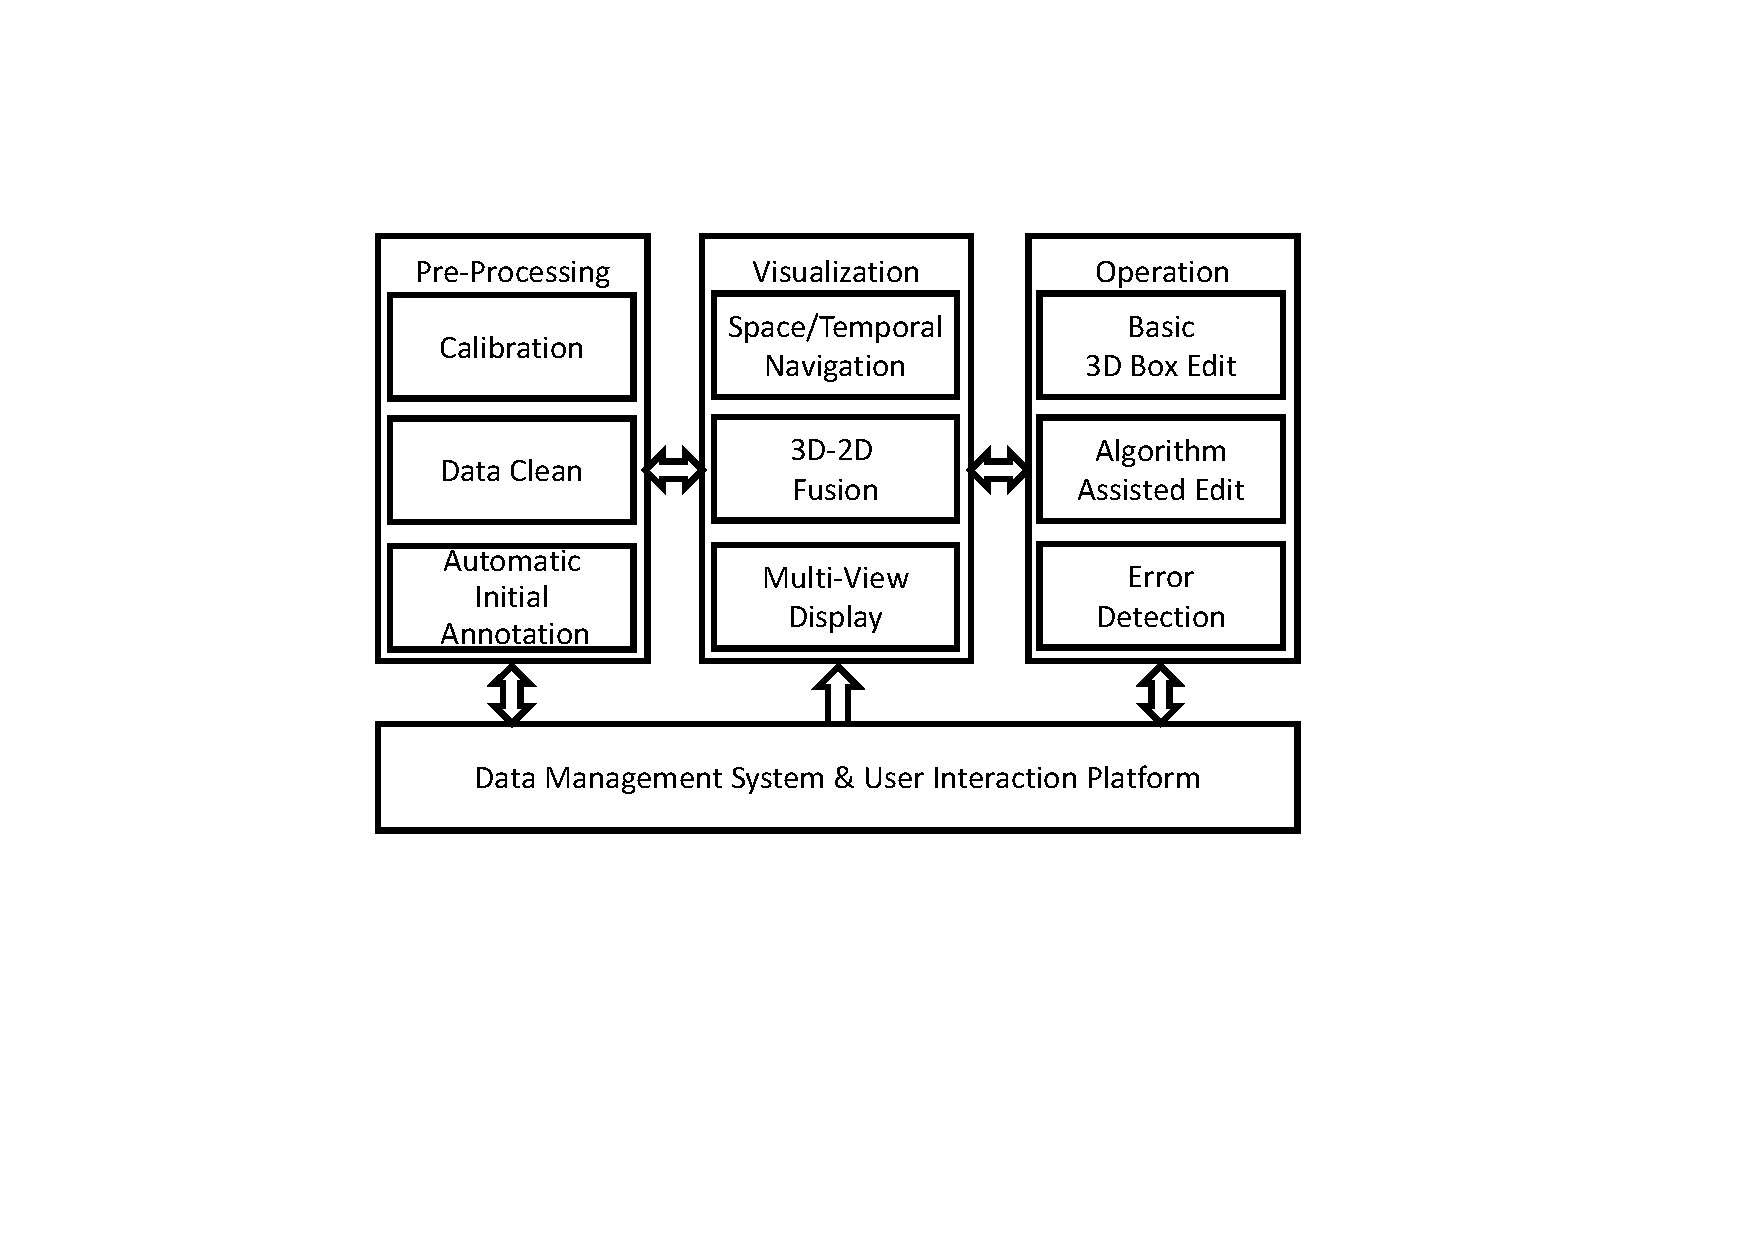
\includegraphics[width=0.45\textwidth]{./figures/arch}\\ %\vspace{-0.3cm}
  \caption{An illustration of our annotation platform. Our annotation procedure includes 3 modules, which are pre-processing, visualization and operation, respectively. The pre-processing module is used to obtain the sensor calibration information, filter the noises in data, and initialize AI method-based annotation results. The visualization module is utilized to assist data annotation. And the operation module implements the 3D bounding box annotation in the point clouds with algorithm assistance and also checks the annotation error.}
     \label{fig:main_ui}
     \vspace{-0.3cm}
\end{figure}

\begin{enumerate}
  \item Irregular density point cloud. In practical, the density of point clouds depends on distance between the sensor and measured objects, sensor type, and reflectivity of the measured objects, etc. Therefore, how to solve the different density of point clouds, including sparse and dense, becomes crucial.
  \item High-precision annotation. Compared with 2D image annotation, the annotation information of 3D point clouds becomes more complexity. It includes scale at each dimensionality axis, and heading angle of the object. How to obtain the accurate annotation information becomes important.
  \item Rich categories of object. The data-driven-based methods can distill the knowledge from the rich categories of the dataset, so that these methods can keep the favorable performance. The number of these objects is numerous. How to quickly annotate and balance these objects is also a critical issue.
  \item Reasonable data structure. The reasonable annotation data structure can efficiently decrease the store space and boost the speed of access.
  \item Flexible tool. Labeling the 3D objects is an enormous work, which includes annotation large amounts of objects and operation instructions for users. Therefore, developing a flexible labeling tool is much more important.
\end{enumerate}

The resolution of 3D point clouds is a formidable limitation for 3D annotation. Each frame point clouds obtained by LiDAR, like Velodyne, RoboSense, etc., has at least 10K 3D points. The measurement radius of  LiDAR is larger than 150 meters. So there are quite a few objects with a small number of points, extremely fewer than 10 points. These low-resolution 3D objects are even beyond the perception ability of humans. Another limitation is how to improve the annotation efficiency of the same object in consecutive frames, especially when the objects being farthest away from the sensor are with low-resolution 3D points.

An flexible annotation tool can improve the annotation efficiency and dataset quality. A considerable amount of research has been done on how to annotate 3D point clouds, like PointAtMe~\cite{pointatme}, LabelMe3D~\cite{LabelMe3D}, etc., during the last decade. The flexible annotation tool should be with easily applicable, intelligible and favorable visibility, as shown in the Fig.~\ref{fig:main_ui}. The intelligible plug-in of the annotation toolkit can promote the speed of the annotation process. The favorable visibility can raise the quality of the dataset, specifically in balancing the number of objects.

In this paper, we propose an efficient 3D point clouds annotation tool, with flexible operation, semi-autonomous annotation, and rapid deployment, to improve the annotation efficiency and assure the dataset quality. The contribution of this work as shown in the following.
\begin{itemize}
  \item Developing a flexible operation annotation tool for 3D point clouds;
  \item Developing a semi-autonomous method to annotate the same objects in the consecutive frames;
  \item Developing an intelligent plug-in being used to count the number and type of labeled objects.
\end{itemize}

The rest of this paper is organized as follows. Section~\ref{Realtedwork} introduces the related work on 3D objects annotation methods.
Section~\ref{setup-statement} describes the system setup and problem statement. Section~\ref{Approach} presents the proposed method.
Section~\ref{result} provides the experiment results and discussions. Section~\ref{conclusions} concludes this paper and outlines future work. To facilitate future research, the code has been released at "\url{http://www.baidu.com}".
\section{Related work}
\label{Realtedwork}
According to the types of annotation equipment, much of the research in the 3D annotation area in recent years can be classified as VR-free (virtual-reality-based) and VR-based methods.
\subsection{VR-free annotation method}
VR-free methods can assure the 3D annotation quality  and are without additional equipments to finish specific annotation tasks.
Details on VR-free methods include the 2D-3D fusion-based and pure 3D-based annotation.
2D-3D fusion-based methods need the accurate spatial transformation relationship between 2D cameras and 3D sensors.
The spatial transformation relationship is calibrated by the stereo-vision algorithms, including Zhang's method~\cite{zhangzhegnyou}, Camera-LiDAR calibration~\cite{roadCalibration}, etc.
But the performance of annotation strongly depends on the 2D-3D correspondence estimated from each sensor data. In addition, the 3D point are discrete and cannot find the accurate corresponding pixels at the image, which can increase the error of calibration and projection. A slice of these methods can only process the specific scenarios, like static scenarios, indoor scenarios, and so on.

Another kind of methods directly operates at the layer of 3D point clouds.
The method proposed by Yu \textit{et al.}~\cite{yu2012efficient} selects some points around the 2D projection of the object in 3D environment, which can approximately annotate the 3D object according to the structure-aware information. The cluster-based methods and segmentation-based method stand for the semi-autonomous and fully autonomous annotation method.
These methods outperform the VR-based annotation methods. However, these methods are with higher time consuming and computation complexity~\cite{pointatme}. It is worth noting that the method~\cite{monica2017multi} is the only one seriously evaluating the speed of their annotation tool. And we also adopt the metric~\cite{monica2017multi} to evaluate the speed of our label tool.
\subsection{VR-based annotation method}
VR equipment is helpful for the 3D environment understanding. It can afford the immersion experience during wearing VR equipment, which can directly show the real environment before the practitioners. Taking advantages of VR, VR-based methods for 3D annotation are proposed in quite a few works~\cite{pointatme,wilkes20123dVR,coffey2011interactiveVR}. These methods use the 6 degree-of-freedom (DoF) device and VR buttons to replace the 2D screen-based or the smartphone functionality-based operations. And these method also acquire the satisfied results. However, the annotated objects by these methods are too coarse to afford the requirements of the practical applications. The VR-based methods depends on the hand gestures and 2 controllers to tune the bounding box of the 3D objects. During the trade-off between efficiency and quality, it is difficult to implement fine-tuning the attitude, size and angle.  The labelled bounding box by the VR-based methods are with bigger errors than that of the VR-free methods.

Another limitation of VR-based methods is the point clouds subject to the same object within an appropriate bounding box.
It needs multiple repeat operations to select the proper boundary points.
Specifically, the labeling process of the complex objects with irregular boundaries, like trees, zebra lines, etc., becomes more difficult than that of other objects with regular boundaries, such as cars, vans, and so on.
These 2 limitations increase the time consuming and decrease the annotation quality of 3D objects.
\subsection{The framework of annotation method}
The framework of annotation method includes explorer-based and software-based. The explorer-based framework is flexible to users for labeling 3D objects, which is based on the elements of the Web page. Therefore, the annotation framework, like LabelMe3D~\cite{LabelMe3D}, our proposed method, etc., can adaptively perform at any computer without additional operations. The software-based methods, like AppoloSuite[], also need additional component that can ensure to execute. And it is difficult to synchronously and instantly update, which maybe cause the inconsistency of data, or other unpredictable results.

In this work, our proposed method directly annotate the objects at the 3D point clouds layer with the explorer-based framework. Our proposed method can successfully process the trade-off between time-consuming and data-quality.
\section{3D annotation tool}
\label{3D annotation tool}

We follow the principles listed below to create our tool:

\begin{itemize}
	\item the details of an object and its 3d bounding box should be easy to check
	\item the operations to annotate one object should be minimized
	\item human work shall be reused and exploited to reduce the burden of labor
\end{itemize}

\subsection{Visualization}

\subsubsection{Sub-views}
We split the main window into 1 main view and 5 sub-views, as shown in Fig.~\ref{fig:main_ui}. As in \cite{Zimmer20193DBA, more..}, the top/side/front projective views is provided to easily check the box alignment, different from \cite{Zimmer20193DBA} we hide environment points in these views to make it clean. we also provide an extra focused fusion view (bottom left sub-view in \ref{fig:main_ui}) to help check image details easily, otherwise a user will have to zoom in/out the context image.

\subsubsection{fast-toolbox}
When an object is selected (by mouse click, or navigate key shortcut), a floating fast-tool-box shows next to it, as shown in Fig.\ref{fig:main_ui}. A user can change object type, tracking id, activate focus mode, among others.

\subsubsection{focus-mode}
We provide a focus mode to facilitate detail check, as shown in Fig.\ref{fig:focus-mode}. When activated through fast toolbox,the target object is automatically centered and zoomed in, most background hidden, while all editing features still applicable. Without this feature a user has to pan,  zoom and rotate the main view often, which we think is a lot operations and thus laborious.

\begin{figure}[thpb]
	\centering	
	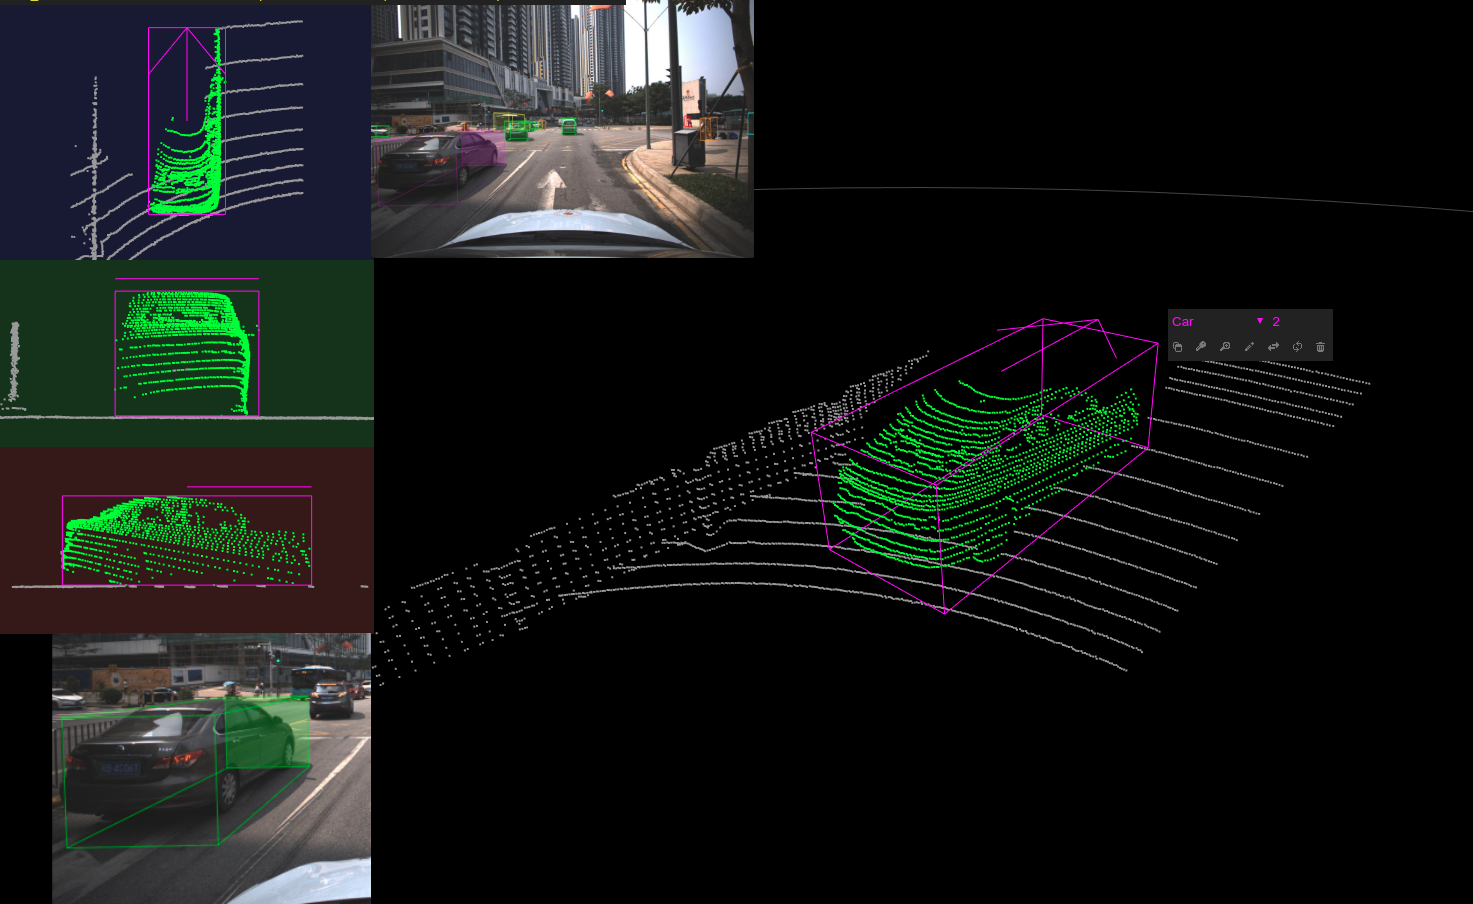
\includegraphics[width=0.9\linewidth]{./figures/focus-mode}\\
	\caption{Focus mode}
	\label{fig:focus-mode}
\end{figure}


\subsubsection{camera auto-switch}
it's common to have multiple cameras and corresponding images to annotate, \cite{Zimmer20193DBA} displays all them on top of the main view, while \cite{} display one of them, we choose the latter way but with an automatic image switching feature. Specifically when an object is selected, the most relevant camera image is displayed, while manual selection is also possible.
note that this feature needs the calibration data to be available.

\subsubsection{coloring}
All boxes and points inside are colored according to their types, and selected object are colored differently.

\subsection{Editing}
In this section we describe the basic editing operation, some advanced algorithm-assisted editing are introduced later.


A box can be created with context menu(triggered by right click), the box dimension is initialized by object category. In main view(Fig.\ref{fig:main_ui}), click a box to select it, click again (or click edit button in fast toolbox) to show/switch the operation handlers (Fig.\ref{fig:box-mouse-edit}), drag the handlers to resize,rotate or move the box, click empty place (or press ESC key) to hide operation handlers or un-select the box.

\begin{figure}[thpb]
	\centering
	\begin{subfigure}{0.3\linewidth}
		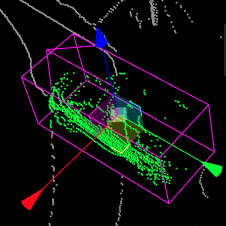
\includegraphics[height=2.5cm]{./figures/box-move}\\
		\caption{move}
	\end{subfigure}
	\begin{subfigure}{0.3\linewidth}
		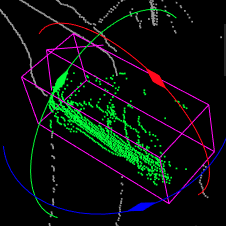
\includegraphics[height=2.5cm]{./figures/box-rotate}\\
		\caption{rotate}
	\end{subfigure}	
	\begin{subfigure}{0.3\linewidth}
		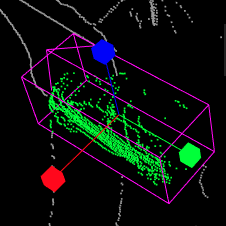
\includegraphics[height=2.5cm]{./figures/box-resize}\\
		\caption{resize}
	\end{subfigure}
	\caption{Box editing in perspective view}
	\label{fig:box-mouse-edit}
\end{figure}

Edit in main view is inconvenient, sometimes you have to change viewpoint for better operation. Actually the annotation is easily and should be checked in the side sub-views, thus we enable editing directly on side sub-views to make a better editing experience. when an object is selected and mouse enters one of the sub-views, the editing is activated automatically on this sub-view. user can drag dotted lines to rotate, resize or move the box, as can be seen in Fig.\ref{fig:box-rotate-in-subview}.

All operations can also be performed by keyboard, and they are summarized in Table \ref{table_keyboard_subview}.

\begin{table}[h]
	\caption{Keyboard Operations on sub-view}
	\label{table_keyboard_subview}
	\begin{center}
		\begin{tabular}{|c|l|}
			\hline
			\textbf{Key} & \textbf{Function}\\			
			\hline
			a & move left\\
			\hline
			s & move down\\
			\hline
			d & move right\\
			\hline
			w & move up\\
			\hline
			q & rotate left\\
			\hline
			e & rotate right\\
			\hline
		\end{tabular}
	\end{center}
\end{table}

\begin{table}[h]
	\caption{Keyboard Operations on main-view}
	\label{table_keyboard_mainview}
	\begin{center}
		\begin{tabular}{|c|l|}
			\hline
			\textbf{Key} & \textbf{Function}\\
			\hline
			1 & select previous object in current frame\\
			\hline
			2 & select next object in current frame\\
			\hline
			3 & previous frame\\
			\hline
			4 & next frame\\
			\hline
			r & rotate box in conter-clockwise(yaw angle)\\
			\hline
			f & rotate box in clockwise(yaw angle)\\
			\hline
			t & reset box\\
			\hline
			g & reverse box direction (yaw angle)\\
			\hline
			v & switch editing mode(Fig.\ref{fig:box-mouse-edit})\\
			\hline
			Ctrl+s & save\\
			\hline
			Ctrl+c & copy reference box (semi-auto annotation \ref{semi-auto-anno})\\
			\hline
			Ctrl+z & undo\\
			\hline
			Ctrl+y & redo\\
			\hline
		\end{tabular}
	\end{center}
\end{table}

\subsection{Assistant algorithms}

\subsubsection{Semi-auto annotation}
\label{semi-auto-anno}
In autonomous driving scenario, data sets are often organized by scenes\cite{Caesar2019nuScenesAM,Patil2019TheHD,lyft2019}, a scene is a sequence of frames shot at one continuous period of time. There are much similarities between neighboring frames, which makes it possible to transfer annotations among them. \cite{Zimmer20193DBA} copies annotations to next frame directly and let user do the adjustment.\cite{Wang2019LATTEAL} uses box estimation algorithm to automatically adjust the box, reusing previous annotated object size if appropriate. Our tool takes this way further by invoking registration algorithm \cite{Yang2016GoICPAG} to automatically adjust the position and rotation, reusing both the size and rotation previously annotated. In most cases our method produces  accurate enough annotation result.


\subsubsection{Auto-shrink}

Due to the unavoidable granularity of adjustment operations (of both keyboard and mouse), it's hard to determine precisely the border of a bounding box, our tool solves this problem by automatically shrink the borders to nearest inner points.

The user can drag the border or corner of a box to enclose all points of the object, after releasing the mouse key, the borders will automatically shrink to best positions.

\subsubsection{Boundary-aware rotation}

When annotate an object we normally perform the following 2 steps iteratively:
\begin{itemize}
	\item adjust position and/or scale
	\item adjust rotation	
\end{itemize}

When we rotate the box, some interior points may go outside(Fig.\ref{fig:boundary-aware-rotation}), obviously it's better keep these points interior while adjust the dimension and/or position automatically, such that we don't have to adjust the dimension and/or position again. We emphasize that \emph{with this feature, to annotate an object is as easy as to enclose all points first and then rotate once}.


\begin{figure}[ht]
	\centering
	\begin{subfigure}[t]{0.2\linewidth}
		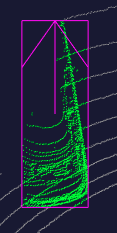
\includegraphics[height=4cm]{./figures/points-enclosed}
		\caption{}

	\end{subfigure}\hfill
	\begin{subfigure}[t]{0.2\linewidth}
		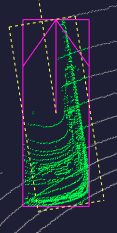
\includegraphics[height=4cm]{./figures/adjust-naively}
		\caption{}
		\label{fig:box-rotate-in-subview}
	\end{subfigure}\hfill
	\begin{subfigure}[t]{0.2\linewidth}
		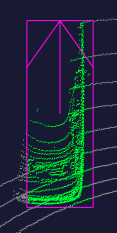
\includegraphics[height=4cm]{./figures/rotate-fail}
		\caption{}
	\end{subfigure}\hfill
	\begin{subfigure}[t]{0.2\linewidth}
		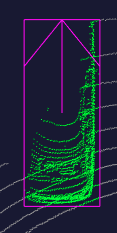
\includegraphics[height=4cm]{./figures/rotate-success}
		\caption{}
	\end{subfigure}\hfill
	\caption{For box in (a), which encloses all points of a car (easily done with auto-shrink operation), if we rotate it counter-clockwise to adjust the heading direction(b), part of the object will go outside(c), our tool can automatically adjust the dimension of the box as shown in (d)}
	\label{fig:boundary-aware-rotation}
\end{figure}


\subsubsection{Prototype-based box initialization}

we use popup context menu to start annotating a new object, when user click object type name, a box is placed at the clicked position (center part of\ref{hptb}), the dimension is set according to the object type, and the heading direction(z-axis rotation) is set upward along the main view (better if the main view is rotated properly beforehand).
A euclidean distance based expansion algorithm is invoked to adjust the box to enclose all points of the same object. By this way the initial bounding box is almost ready.

\subsubsection{Calibration fine-tuning}

\section{Implementation}
\label{Implementation}

\subsection{System Architecture}
We use web-based architecture, the raw data to be annotated is located in server. The end user can start working with a web browser and don't have to download the data set beforehand. The web server is implemented in Python and relies on CherryPy web framework\cite{cherrypy}. For front-end relies on \texttt{WebGL} library Three.js\cite{threejs}.

In server, the raw data is organized by scenes, the directory structure is as in Fig.\ref{fig:data-dir}.

\begin{figure}

\dirtree{%
	.1 data.
	.2 scene1.
	  .3 lidar.
	     .4 frame0000.pcd.
	     .4 ....
	  .3 image.
	    .4 left-camera.
	      .5 frame0000.png.
	      .5 ....
	    .4 front.
	      .5 frame0000.png.
	      .5 ....
	    .4 ....
	  .3 calib.
	    .4 left-camera.json.
	    .4 front.json.
	    .4 ....
	  .3 label.
	    .5 frame0000.json.
	    .5 ....
	.2 scene2.
	   .3 ....
	.2 ....
}
\caption{Raw data organization. The `label` folder is used to store annotation result. the `calib` folder stores lidar-camera calibration parameters, which is optional but requrired for 3d-2d fusion features. We list 3 cameras as an example, more cameras are also supported.}
\label{fig:data-dir}
\end{figure}



\subsection{Semi-auto annotation algorithm}

Semi-auto annotation of our tool is roughly a method to transfer annotation between frames, more accurately than naive paste or liner interpolation. The user need to first select (copy) a reference box, then paste it in appropriate position in target frame. A registration algorithm is invoked to compute the relative transform relation between the reference and target object, the target box is adjusted by the same transform relation. Note that the user need only to paste the box on the roughly right position.


\begin{figure}[htpb]
	\centering
	\begin{subfigure}[t]{0.18\linewidth}
		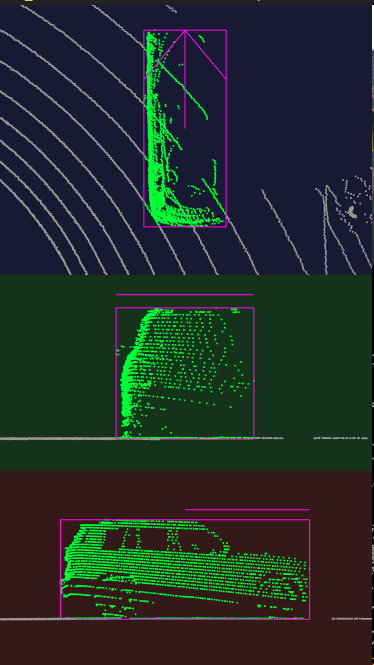
\includegraphics[height=3cm]{./figures/reg-ref-3d}\\
		\caption{}\label{fig:box-ref}
	\end{subfigure}\hfill
	~
	\begin{subfigure}[t]{0.18\linewidth}
		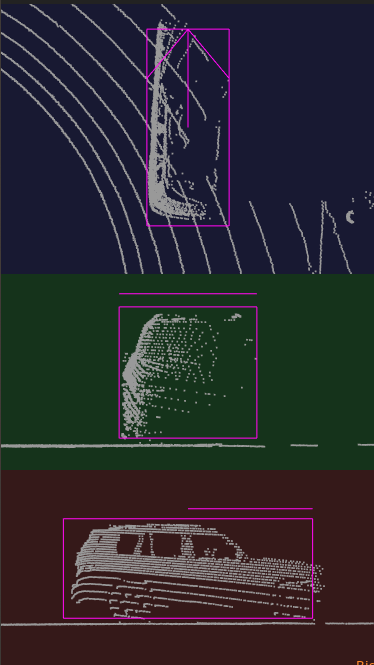
\includegraphics[height=3cm]{./figures/reg-input-3d}\\
		\caption{}\label{fig:box-source}
	\end{subfigure}\hfill
	~
	\begin{subfigure}[t]{0.18\linewidth}
		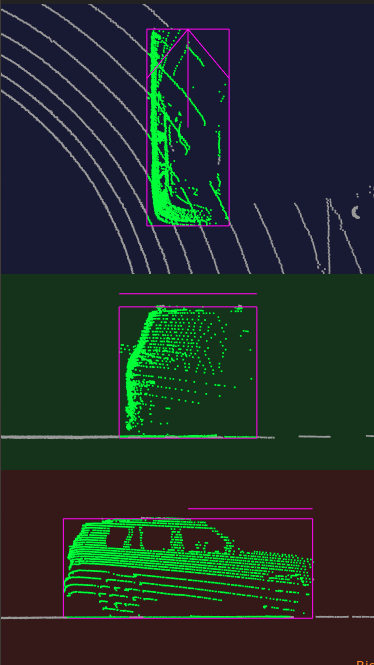
\includegraphics[height=3cm]{./figures/reg-result-3d}\\
		\caption{}\label{fig:box-output}
	\end{subfigure}\hfill
	
	\begin{subfigure}[t]{0.18\linewidth}
		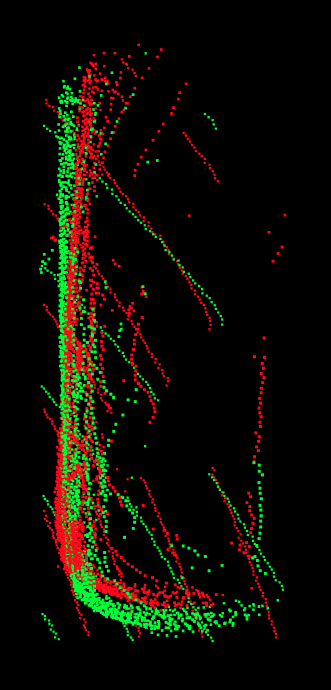
\includegraphics[height=3cm]{./figures/reg-input}\\
		\caption{}\label{fig:reg-input}
	\end{subfigure}\hfill
	~
	\begin{subfigure}[t]{0.18\linewidth}
		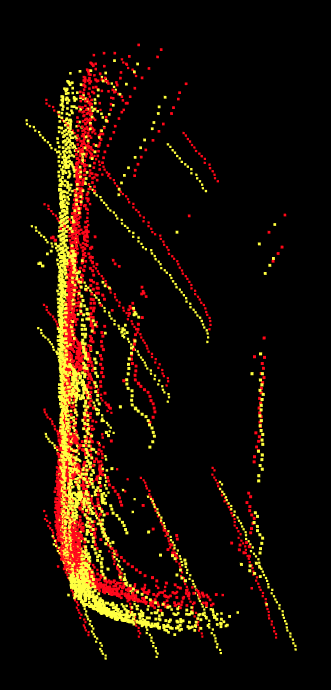
\includegraphics[height=3cm]{./figures/reg-tran}\\
		\caption{}\label{fig:reg-tran}
	\end{subfigure}\hfill
	~
	\begin{subfigure}[t]{0.18\linewidth}
		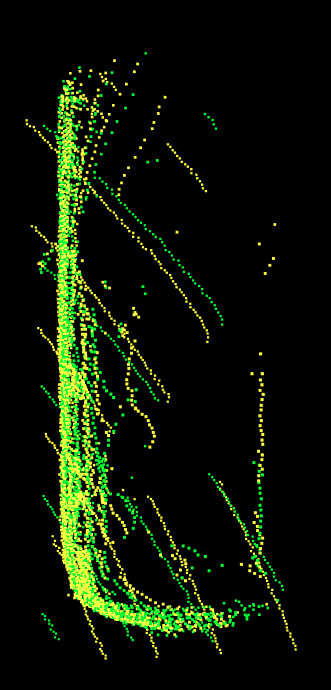
\includegraphics[height=3cm]{./figures/reg-result}\\
		\caption{}\label{fig:reg-output}
	\end{subfigure}\hfill

	
	\caption{Registration based bounding box transfer. \ref{fig:box-ref} is the reference object and its bounding box, \ref{fig:box-source} is the object in another frame with a initial  bounding box, \ref{fig:box-output} is the effect of box being adjusted.}
\end{figure}


Given source and target objects (denoted by $\mathcal{S,T}$ respectively)and their bounding boxes ($b_s,b_t$), a registration algorithm finds the transform matrix $T$ to match $\mathcal{S}$ with $\mathcal{T}$ , minimizing a distance function $dist$,
$$dist(T(\mathcal{S}),\mathcal{T})$$
where we represent points of $\mathcal{S,T}$ in their corresponding bounding box coordinates $B_s$ and $B_t$, the world coordinate system is denoted as $B_w$,

Assume point $s \in \mathcal{S}$ corresponds to $t \in \mathcal{T}$ after registration, then


\begin{align}
T s^{B_s} &= t^{B_t}\\
T B_s^{-1}s &= t^{B_t} \label{eq:eq1}
\end{align}

where $s^{B_s}$ means s represented in $B_s$ coordinate system, $s$ without upper index means default world coordinate system.

If we denote the new coordinate system of $\mathcal{S}$ as $B'_s$, then
\begin{equation} \label{eq:eq2}
s^{B'_s} = t^{B_t}
\end{equation}

by \ref{eq:eq1} and \ref{eq:eq2}, we have
\begin{align}
{B'_s} & = (T B_s^{-1})^{-1}\\
       & = B_s T^{-1} \label{eq:eq5}
\end{align}

If we use the reference object as target, object under annotation as source, (\ref{eq:eq5}) tells us we should apply the reverse transform of registration to the coordinates system, that is, to the box.


\subsection{Boundary-aware rotation}

A naive implementation is to recalculate the dimension of all original interior points and adjust the box accordingly, but it may fail when ground plane is present, after several rotation the box may become too big. One solution is to remove ground plane beforehand, but no algorithm can do this work perfectly as of our best knowledge, especially when the ground is not smooth (as can be seen often in KITTI data set\cite{Geiger2012CVPR} where many cars park on roadside). We use a simple yet effective method to tackle this problem. Specifically, we just ignore the most bottom part (0.1m by default) of the object when calculating the box dimension. Since a user is annotating the object, the pose of the object must be already roughly correct, so the bottom part can filter out ground points effectively. In the other hand, the object dimension estimation is not affected since almost all objects are much higher than 0.1m in traffic scenarios.


\section{Experiment and Evaluation}
\label {Metrics}

\section{USING THE TEMPLATE}
\label{result}

\section{CONCLUSIONS}
\label{conclusions}
A conclusion section is not required. Although a conclusion may review the main points of the paper, do not replicate the abstract as the conclusion. A conclusion might elaborate on the importance of the work or suggest applications and extensions.

\addtolength{\textheight}{-12cm}   % This command serves to balance the column lengths
                                  % on the last page of the document manually. It shortens
                                  % the textheight of the last page by a suitable amount.
                                  % This command does not take effect until the next page
                                  % so it should come on the page before the last. Make
                                  % sure that you do not shorten the textheight too much.

%%%%%%%%%%%%%%%%%%%%%%%%%%%%%%%%%%%%%%%%%%%%%%%%%%%%%%%%%%%%%%%%%%%%%%%%%%%%%%%%



%%%%%%%%%%%%%%%%%%%%%%%%%%%%%%%%%%%%%%%%%%%%%%%%%%%%%%%%%%%%%%%%%%%%%%%%%%%%%%%%



%%%%%%%%%%%%%%%%%%%%%%%%%%%%%%%%%%%%%%%%%%%%%%%%%%%%%%%%%%%%%%%%%%%%%%%%%%%%%%%%
\section*{APPENDIX}

Appendixes should appear before the acknowledgment.

\section*{ACKNOWLEDGMENT}

%%%%%%%%%%%%%%%%%%%%%%%%%%%%%%%%%%%%%%%%%%%%%%%%%%%%%%%%%%%%%%%%%%%%%%%%%%%%%%%%

References are important to the reader; therefore, each citation must be complete and correct. If at all possible, references should be commonly available publications.

\bibliographystyle{IEEEtran}
\bibliography{MyReference}
\end{document}
